% This is the Reed College LaTeX thesis template. Most of the work 
% for the document class was done by Sam Noble (SN), as well as this
% template. Later comments etc. by Ben Salzberg (BTS). Additional
% restructuring and APA support by Jess Youngberg (JY).
% Your comments and suggestions are more than welcome; please email
% them to cus@reed.edu
%
% See http://web.reed.edu/cis/help/latex.html for help. There are a 
% great bunch of help pages there, with notes on
% getting started, bibtex, etc. Go there and read it if you're not
% already familiar with LaTeX.
%
% Any line that starts with a percent symbol is a comment. 
% They won't show up in the document, and are useful for notes 
% to yourself and explaining commands. 
% Commenting also removes a line from the document; 
% very handy for troubleshooting problems. -BTS

% As far as I know, this follows the requirements laid out in 
% the 2002-2003 Senior Handbook. Ask a librarian to check the 
% document before binding. -SN

%%
%% Preamble
%%
% \documentclass{<something>} must begin each LaTeX document
\documentclass[12pt,twoside]{reedthesis}
\setcounter{secnumdepth}{0}
% Packages are extensions to the basic LaTeX functions. Whatever you
% want to typeset, there is probably a package out there for it.
% Chemistry (chemtex), screenplays, you name it.
% Check out CTAN to see: http://www.ctan.org/
%%
\usepackage{graphicx,latexsym} 
\usepackage{amssymb,amsthm,amsmath}
\usepackage{longtable,booktabs,setspace} 
\usepackage{chemarr} %% Useful for one reaction arrow, useless if you're not a chem major
\usepackage[hyphens]{url}
\usepackage{rotating}
\usepackage{natbib}
% Comment out the natbib line above and uncomment the following two lines to use the new 
% biblatex-chicago style, for Chicago A. Also make some changes at the end where the 
% bibliography is included. 
%\usepackage{biblatex-chicago}
%\bibliography{thesis}

% \usepackage{times} % other fonts are available like times, bookman, charter, palatino

\title{Narrative Listening and Intuitions about Composer Identity}
\author{Sarah Wu}
% The month and year that you submit your FINAL draft TO THE LIBRARY (May or December)
\date{May 2023}
\division{Philosophy, Religion, Psychology, and Linguistics}
\advisor{Kevin J. Holmes}
%If you have two advisors for some reason, you can use the following
%\altadvisor{Your Other Advisor}
%%% Remember to use the correct department!
\department{Psychology}
% if you're writing a thesis in an interdisciplinary major,
% uncomment the line below and change the text as appropriate.
% check the Senior Handbook if unsure.
%\thedivisionof{The Established Interdisciplinary Committee for}
% if you want the approval page to say "Approved for the Committee",
% uncomment the next line
%\approvedforthe{Committee}

\setlength{\parskip}{0pt}
%%
%% End Preamble
%%
%% The fun begins:
\begin{document}

  \maketitle
  \frontmatter % this stuff will be roman-numbered
  \pagestyle{empty} % this removes page numbers from the frontmatter

% Acknowledgements (Acceptable American spelling) are optional
% So are Acknowledgments (proper English spelling)
    \chapter*{Acknowledgements}
	To my parents—thank you for supporting me throughout my education and for fostering my curiosity. To my thesis advisor Kevin Holmes—I'm grateful for your mentorship. Thank you for all your engaging lectures and classroom discussions and opportunities to conduct psychological research. To Harrison—we made it to another graduation together! Thank you for your sweet dedication to the Sarah Wu club and all that entails. To all my music teachers—thank you for pushing me to search for the story in the music.
	

% The preface is optional
% To remove it, comment it out or delete it.
    % \chapter*{Preface}
	% This is an example of a thesis setup to use the reed thesis document class.
	
	

    % \chapter*{List of Abbreviations}
	% 	You can always change the way your abbreviations are formatted. Play around with it yourself, use tables, or come to CUS if you'd like to change the way it looks. You can also completely remove this chapter if you have no need for a list of abbreviations. Here is an example of what this could look like:

	% \begin{table}[h]
	% \centering % You could remove this to move table to the left
	% \begin{tabular}{ll}
	% 	\textbf{ABC}  	&  American Broadcasting Company \\
	% 	\textbf{CBS}  	&  Columbia Broadcasting System\\
	% 	\textbf{CDC}  	&  Center for Disease Control \\
	% 	\textbf{CIA}  	&  Central Intelligence Agency\\
	% 	\textbf{CLBR} 	&  Center for Life Beyond Reed\\
	% 	\textbf{CUS}  	&  Computer User Services\\
	% 	\textbf{FBI}  	&  Federal Bureau of Investigation\\
	% 	\textbf{NBC}  	&  National Broadcasting Corporation\\
	% \end{tabular}
	% \end{table}
	

    \tableofcontents
% if you want a list of tables, optional
    \listoftables
% if you want a list of figures, also optional
    \listoffigures

% The abstract is not required if you're writing a creative thesis (but aren't they all?)
% If your abstract is longer than a page, there may be a formatting issue.
    \chapter*{Abstract}
	People exhibit a robust tendency to imagine stories when listening to music (i.e., narrative listening), which could be driven by features of the music itself or external factors like beliefs about the composer. Across two studies, the present thesis examined the role of the latter, specifically the relationship between beliefs about human and AI composers and narrative listening. In Study 1, participants listened to six clips of instrumental music, provided narrative listening responses, rated the perceived intentionality of the composer, and judged whether they thought the music was composed by a human or an AI system. In Study 2, composer identity beliefs were experimentally manipulated using a within-subjects design, such that each piece of music from Study 1 was preceded by information describing its creation by a human or an AI system. The results provide evidence that composer identity beliefs are correlated with perceptions of musical narrative, but fall short of showing that they causally impact them. Across studies, perceived intentionality seemed to mediate this relationship. Implications for narrative processing and AI research are discussed. 
	
	
	% \chapter*{Dedication}
	% You can have a dedication here if you wish.

  \mainmatter % here the regular arabic numbering starts
  \pagestyle{fancyplain} % turns page numbering back on

%The \introduction command is provided as a convenience.
%if you want special chapter formatting, you'll probably want to avoid using it altogether

    \chapter*{Introduction}
         \addcontentsline{toc}{chapter}{Introduction}
	\chaptermark{Introduction}
	\markboth{Introduction}{Introduction}
	% The three lines above are to make sure that the headers are right, that the intro gets included in the table of contents, and that it doesn't get numbered 1 so that chapter one is 1.

% Double spacing: if you want to double space, or one and a half 
% space, uncomment one of the following lines. You can go back to 
% single spacing with the \singlespacing command.
% \onehalfspacing
\doublespacing

Listeners readily imagine stories when listening to music, even in the absence of lyrics. This propensity may be part of a broader human tendency to identify patterns or derive meaning from abstract stimuli. For example, classic studies have demonstrated that people perceive shapes moving in arbitrary patterns as agentic entities (Heider \& Simmel, 1944; Geraci \& Simion, 2021). When watching even brief animations of these shapes, people cannot help but view them as characters in a story, with motivations and emotions. In the case of music, listeners may consider salient features such as timbre and pitch to mentally construct a narrative. But the features of the music itself may not be the sole determinant of the listening experience. Aesthetic judgments of music are influenced by, among other factors, beliefs about the title of the piece (Anglada-Tort et al., 2019; Simonton, 1995), the prestige of the composer (Fischinger et al., 2018), and visual imagery that the piece evokes (Vuoskoski \& Eerola, 2015). 

Yet another factor that may contribute to music perception is knowledge about a piece’s conception. Research on experimental aesthetics suggests that observers consider the intentionality behind works of art (Jucker et al., 2014; Pelowski et al., 2017). For example, people tend to give higher ratings of artistic merit to a blurry photograph of flowers when told that the photographer deliberately used defocusing to accentuate the vibrant character of the flowers than when told that the photographer simply forgot to focus the lens (Jucker et al., 2014). Even young children take intentionality into account. In one classic study, 3- and 4-year-old children assigned different names to a drawing when told it was created intentionally than accidentally (Bloom \& Markson, 1998). Together, these findings suggest that beliefs about the intention of the artist are central to evaluating the identity, validity, and impact of the art. 

Questions of intentionality in art have become especially relevant in the past few years because of rapid advances in the field of artificial intelligence (AI). Trained on data consisting of millions of human-created artworks, AI algorithms can identify perceptual patterns that make up a variety of artistic genres and styles. Using these algorithms, AI systems can produce their own art in similar styles. With a simple text prompt, users can quickly generate art that looks convincingly human. However, these artworks may not be appraised as having the same artistic merit as those believed to have human origin (Chamberlain et al., 2018; Hong et al., 2022). For example, Chamberlain et al. (2018) found that images thought to be human-created were judged more aesthetically valuable than those thought to be computer-created, even though the two types of images were discriminated at levels barely above chance. 

If people attribute less intention to computers than humans and judge computer-created artworks less valuable as a result, this may have important implications for music perception. Computer-composed music may be less likely than human-composed music to be perceived as having a coherent structure or message, and thus may less readily elicit imagined narratives. The present thesis examines whether people’s tendency to narrativize when listening to music depends on whom they believe the composer to be: a human or a computer.

\section{The Physical Stance}
The human brain is wired for pattern recognition. In the context of music, this involves tracking various acoustic properties, such as timbre and pitch, and generating predictions about what sounds will come next (Salimpoor et al., 2015). The act of processing music based on its physical properties aligns with the philosophical concept of the physical stance (Dennett, 1989). When people adopt the physical stance, they use information about the physical properties of an entity to make predictions about its future behavior. For example, in Western music certain combinations of pitches are more likely to occur than others. Based on learned associations from previous exposure to Western music, listeners can accurately predict upcoming chords. 

Music varies on many dimensions that may collectively be associated with certain events in the environment—what music theorists refer to as topicality. For instance, in film a series of harp arpeggios is conventionally used to signal the transition to a dream sequence. This particular combination of pitch and timbre alone may come to evoke dream-related scenes in the listener’s mind. A piece of music can also include different degrees of contrast when salient features change over the course of its duration. Given that feature changes often coincide with the perceived boundaries of events in the environment (Hard et al., 2019), the features of a musical piece alone may be sufficient to elicit an imagined narrative. Such links between stimulus features and narrative listening would support a low-level, bottom-up account of music perception. However, this explanation may not fully account for the propensity to narrativize music. 

\section{The Intentional Stance}
Another predictive strategy that may be at play when listening to music is the intentional stance: the ascription of mental states to an entity (Marchesi et al., 2019). When adopting the intentional stance, people assume that an observed agent acts in line with its goals, intentions, or beliefs (Pantelis et al., 2015). Evidence for this strategy comes from studies in which participants are led to form beliefs about the origins of simple perceptual stimuli. Typically, some participants are told that the stimuli were derived from an intentional agent (e.g., a human), while others are told that they were derived from an unintentional agent (e.g., a computer). Such beliefs about intentionality are often pitted against physical features of the stimuli, which are also experimentally manipulated.

This approach has been employed to study which type of information—intentions or physical features—is relied on more heavily for predictive action. In a study by Stanley et al. (2007), participants were led to believe that a dot’s trajectory was either biological (based on human movements) or nonbiological (generated by a computer), and the dot’s actual motion profile either matched participants’ beliefs or did not. Participants were asked to move their arm in time with the dot’s movements. The outcome of interest was motor interference: the tendency to mirror incompatible movements (e.g., those perpendicular to one’s own) less precisely than compatible movements (e.g., those parallel to one’s own). If physical features are more important for predictive action, interference effects should be stronger when the dot moves like a biological entity, regardless of participants’ beliefs about what generated the motion. However, if such beliefs are more important, interference effects should be stronger when participants believe the motion is biological, regardless of the actual motion profile. The results supported the latter prediction, suggesting that intentionality can be more influential than physical features when generating predictions—a kind of top-down effect on perception (Lupyan et al., 2020). 

Such top-down effects have neural signatures. In an fMRI study by Abu-Akel et al. (2020), participants played a competitive game against an unseen opponent that they believed was either a human or a computer responding intentionally or unintentionally (i.e., following a script). In reality, the opponent was always a computer program that generated moves at random. Even so, activity in the “mentalizing network” of the brain—a circuit comprising the temporoparietal junction and the anterior paracingulate cortex—was observed when participants believed they were competing against an intentional agent, whether human or computer. Conversely, these regions of the brain did not show activity when participants believed the opponent was responding without intention. These results have two main implications. For one, they suggest that intentionality is distinct from the entity producing the intentional behavior (human or computer). Relatedly, they demonstrate that computers need not be assumed to be unintentional, contrary to previous studies that have made this assumption when comparing participants’ reactions to humans and computers.  

\section{The Role of Intention in Aesthetic Judgments
}
With regard to music perception, listeners may adopt the intentional stance by inferring the mental state of the composer and assuming they created their music for a reason. Research in experimental aesthetics supports this possibility. When people perceive art, they are sensitive to a host of cues beyond the art itself (Pelowski et al., 2017). Jucker et al. (2014) specifically investigated the role of perceived intention because of its potential to elucidate the meaning of works of art. As a given work is often ambiguous, the most direct way to understand its purpose is to defer to the creator’s intention. 

To test this phenomenon, Jucker et al. (2014) paired artistic stimuli with statements that varied the artist’s level of intentionality. For example, after viewing a white canvas covered entirely with colored dots, some participants read that the artist produced it spontaneously as a way to relax herself between projects (a low-intention cover story), while others read that the artist had exclusively created this type of piece for years, deriving gratification from combining colors in infinite ways (a high-intention cover story). Stimuli were less likely to be perceived as art and less likely to deem it worthy of an art exhibition when they were accompanied by low-intention cover stories than high-intention cover stories. These results suggest that viewers weigh the intention behind a work of art when judging its merit, at least when information about intention is made explicitly available. 

People also invoke intention spontaneously when explaining their aesthetic preferences. In studies by Hawley-Dolan and Winner (2011), participants were presented with pairs of highly similar abstract paintings, one by a professional expressionist and the other by either a child or an animal. Participants were asked to select which painting they liked more and which one they thought was a better work of art. For each selection, participants were prompted to explain their choice, and their response was coded as “mentalistic” or “nonmentalistic.” Mentalistic responses referred to the skill, thinking, or intentionality of the artist (e.g., “the second one looks more thought out”), while nonmentalistic responses referred to the content of the images (e.g., “because it has simple colors”). Despite the visual similarity of the images, participants preferred professional paintings, judged them as better than non-professional paintings, and gave more mentalistic responses when justifying their selection of them. This tendency to offer mentalistic rationales suggests that people readily infer intention behind works of art. 

\section{Art Produced by Artificial Intelligence
}
Art produced by computers may be less likely to induce the intentional stance. Indeed, in the 1950s, Lejaren Hiller—the pioneer of computer-composed music—emphasized that his goal when composing music with a computer was not to convey emotions to the listener. Rather, he used a computer to understand the “objective” features of the music, separate from the relationship between composer and listener (Hiller, 1959). To do so, a high-speed computer generated random integers—the machine-readable equivalent of musical notes—which were then screened by mathematical algorithms that specified conventional rules of music composition (Hiller \& Isaacson, 1958). Hiller and his colleague Leonard Isaacson tested these algorithms in a series of experiments, eventually creating a string quartet. Today, AI music generators can create their own music by detecting patterns among the music they are trained on (Dhariwal et al., 2020). At the same time, they have limitations that prevent them from sounding perfectly human-like. Many of them cannot, for example, capture subtleties in timbre and dynamics that are essential for an authentic sound (Dhariwal et al., 2021; Oore et al., 2020). 

To date, AI has been more successful in the domain of visual art. The outputs of AI art generators offer concrete examples of the artistic capabilities of computers. These systems are trained on millions of images of human-created art, and their algorithms recognize a myriad of patterns in those images. With enough training, they can generate their own images in similar styles (Ramesh et al., 2021). Certain AI systems, such as DALL-E 2, accept text input from a user to generate images in a range of media. Figure ~\ref{fig-tired-student} shows examples of novel images generated by DALL-E 2 in response to a user’s text prompt. To produce these images, DALL-E 2 had to “understand” the individual concepts of “tired,” “student,” and “working,” as well as the relationships between those concepts. Then it had to incorporate the style specification “oil painting” to render the image in what looks like brush strokes, with shading included to enhance the realism. 

These AI systems are not limited to generating depictions of the real world, but can also generate abstract or surreal images by combining user-provided concepts in original ways. For each generated image, several variations can also be generated, all in a matter of seconds. Thus, AI systems have the power to produce art that is both familiar and unexpected (Kelly, 2022).

\begin{figure}
\centering
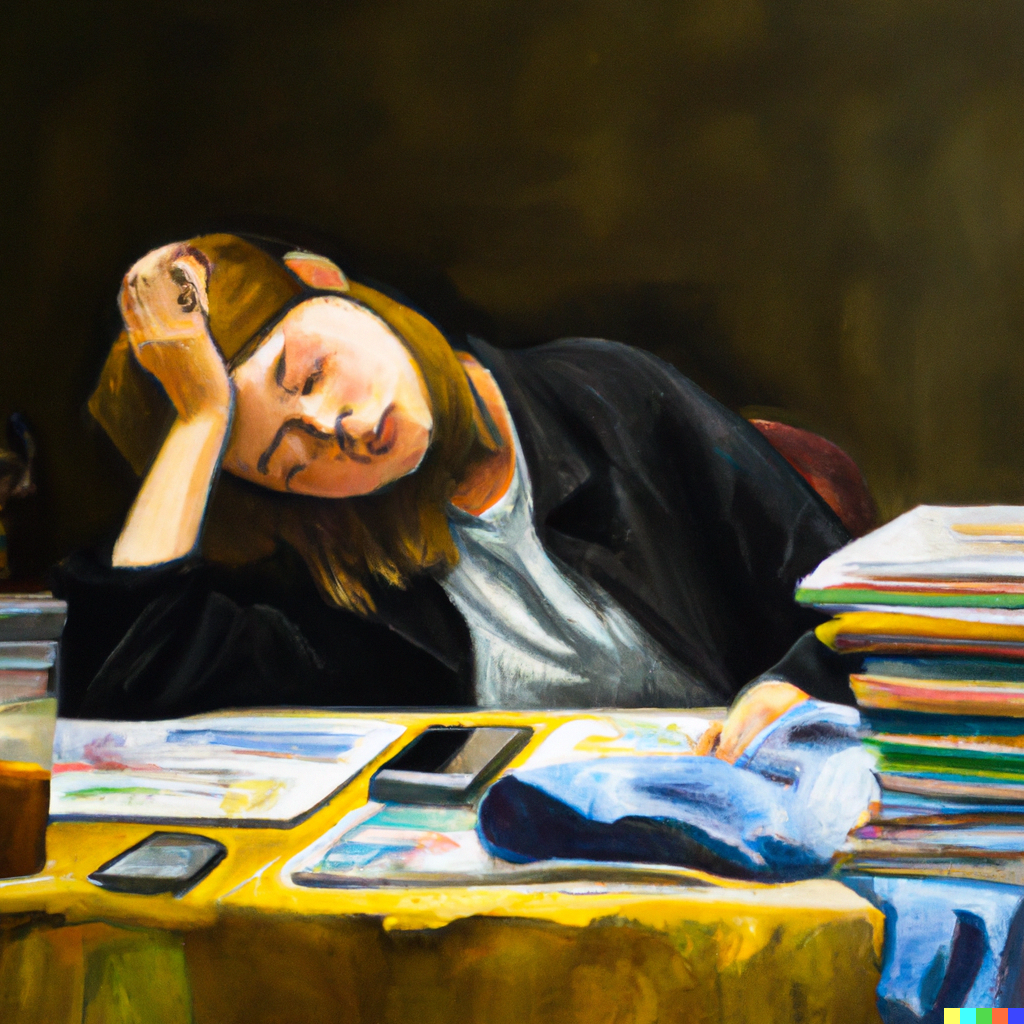
\includegraphics[scale=0.15]{DALLE_tired_student}
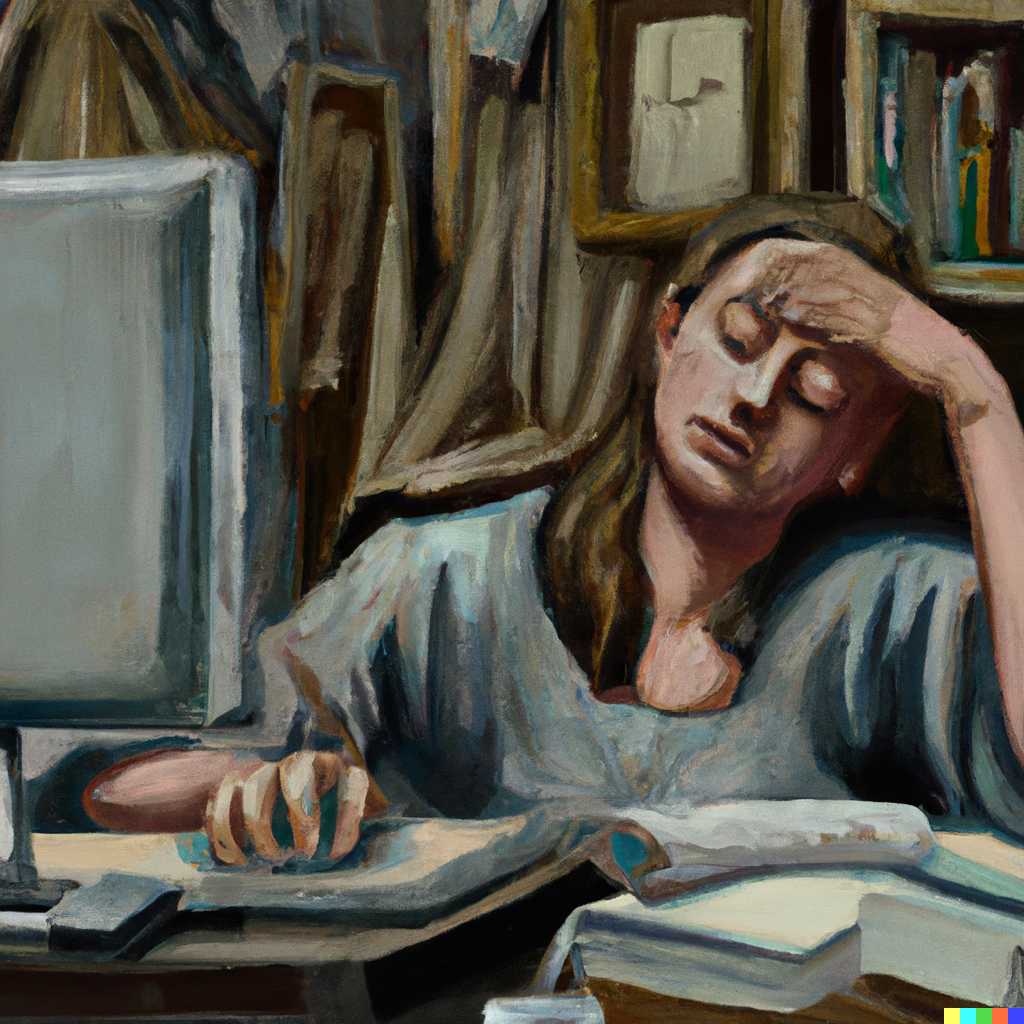
\includegraphics[scale=0.15]{DALLE_tired_student1.png}
\caption{DALL-E 2 images generated from the text prompt “a tired student working on her undergraduate thesis, oil painting.”}
\label{fig-tired-student}
\end{figure}

These systems are not without controversy. Recently, digital artist James Allen faced backlash for using AI to win an art competition (Roose, 2022), sparking debate about the role of human creativity in art and the potential obsolescence of human artists. Art is one of many domains in which AI rivals or even outperforms human efforts. The impressive outputs of AI art generators have forced artists and the general public to consider what roles human and computer artists play in society. If each type of artist can produce art autonomously, and of similar quality, it would seem as though they should be able to fill the same role. However, the “autonomy” of an AI system is difficult to define because AI algorithms require at least some human involvement (Hong et al., 2020). For example, AI art generators are programmed by using human-created art as training data, which is why some critics rebuked Allen for “high-tech plagiarism” (Roose, 2022). At the same time, once an AI system has been trained on enough data, it can exhibit human-like “creativity,” generating innovative ideas that exceed its input (Boden, 1998). 

\section{Reactions to Computer-Generated Art and Music
}

A growing body of research has examined whether knowing that a work of art was created by a human or a computer affects the way it is perceived. A number of studies have found that when people believe the work was created by a human, they often exhibit stronger, more positive reactions toward it (Chamberlain et al., 2018; Grace et al., 2019; Hong et al., 2022; but see Friedman \& Taylor, 2014). For example, participants who read program notes describing a song as human-composed rated its emotional intensity higher than songs described as composed from physiological data (Grace et al., 2019). 

For music that was actually AI-generated, observer reactions depend on the perceived anthropomorphism of the AI system. AI systems that are perceived as musicians, for example, are judged as more aesthetically appealing, more creative, and better crafted (Hong et al., 2022). These judgments could be due to a general preference for human-made products in domains that are high in identity-relevance, like the arts (Morewedge, 2022), or that are regarded as unique to humans (Shank et al., 2022).

There is a neural basis for these effects that points to a role for the intentional stance. In a functional magnetic resonance imaging (fMRI) study by Steinbeis and Koelsch (2009), participants were told they would be presented with musical pieces that had been composed by either a human or a computer, and were asked to focus on their pleasantness. All of the pieces, which were atonal and lacked conventional harmonies, actually had human composers. Nevertheless, pieces believed to be computer-composed elicited different patterns of brain activity than those believed to be human-composed. The latter elicited greater activity in brain areas associated with mental state attribution: the anterior medial frontal cortex (aMFC), the superior temporal sulcus (STS), and the temporoparietal junction (TPJ). In addition, activity in the aMFC was positively correlated with the level of intention participants reported perceiving in the music. 

These findings underscore the power of beliefs about the identity of a composer. Simply perceiving the purported product of a computer or a human—sans direct interaction with the alleged composer—yields observable differences in neural activity and self-reported perceptions. Critically, the perceptual features of Steinbeis and Koelsch’s (2009) musical stimuli did not covary with participants’ beliefs about their origin. It is striking, then, that beliefs and expectations alone can shape the way those features are perceived. 

\section{The Role of Beliefs in Human-Computer Interaction
}

The intentional stance extends to direct interactions with another agent. In a study by Crompton and MacPherson (2019), older adults completed a collaborative learning task with a “partner”—a computer system they were led to believe was controlled by a human or acted autonomously (but was actually human-controlled in both conditions). The only difference between conditions was whether the system had natural or synthetic speech, respectively. Despite the subtlety of this manipulation, there were many observable differences in participants’ behavior. Compared to participants who believed they were interacting with a human, those who believed they were interacting with a computer took longer to complete the task, were less accurate, changed their answers more, and recalled them with less detail. These findings further illustrate the power of beliefs about who (or what) generated a given product or behavior. The experimental manipulation had no effect on the way the computer system functioned, yet participants’ task performance was clearly hindered when they believed they were interacting with a computer. 

Taken together, the research reviewed thus far suggests that both subjective judgments and objective behaviors are subject to the influence of mere beliefs. For works of art—which are inherently subject to interpretation—beliefs about the intentionality of the creator may be especially likely to affect the aesthetic experience. In the domain of music, the listening experience may depend in large part on the level of intention people attribute to the composer. In the following section, I discuss research on a key aspect of the listening experience that may reflect such intentional attributions: narrativity, or the tendency to process music in terms of an imagined story. 

\section{Narrative Listening}

Narrative structure seems like an intrinsic part of music. People cannot help but infer a narrative when listening to certain patterns of sound (Tan \& Kelly, 2004). A series of recent studies by Margulis et al. (2019, 2022a, 2022b) investigated the narrative processing of music in depth. Specifically, these studies examined listeners’ propensity to narrativize using three metrics: narrativity, narrative engagement, and the content of imagined narratives. 

\emph{Narrativity} is the likelihood that a given piece of music will trigger an imagined story. To study this phenomenon, Margulis et al. (2019) presented U.S. and Chinese participants with Western and Chinese classical music and asked them to report whether they imagined a story while listening to each piece. If they did imagine a story, they were prompted to rate their \emph{narrative engagement}through four Likert-scale items assessing the vividness of their perceived narratives (e.g., “I imagined a story with a clear setting, characters, and events”). The results showed that U.S. participants were more likely to imagine a story when listening to Western classical music than Chinese classical music, while Chinese participants showed the opposite pattern. Moreover, when participants imagined a story, they reported higher narrative engagement for the music from their own culture. 

To probe the \emph{content} of participants’ imagined narratives, Margulis et al. (2022b) used the word embedding model word2vec. This model quantifies the semantic similarity of words by considering the context in which the words occur. Its underlying assumption is that words with similar meanings appear in similar contexts (Landauer \& Dumais, 1997; Mikolov et al., 2013). With a large enough corpus of text, word2vec can make highly accurate inferences about the meaning of individual words. For example, the model would infer that “dog” is more similar to “cat” than to “candy” because contexts containing “dog” are more similar to contexts containing “cat” than to contexts containing “candy.” Such inferences are derived by transforming each word into a numerical representation called a word embedding or word vector: a sequence of numbers that uniquely identifies the word based on its frequency and co-occurrences within a corpus. Word vectors are mapped onto a vector space, where words that are more semantically similar are positioned closer to each other. Within this geometric representation, a simple distance metric—cosine similarity—can be used to infer the similarity between any two words. 

Margulis et al. (2022b) applied word2vec to stories imagined when listening to musical pieces. U.S. and Chinese participants (from Arkansas and Michigan, and Dimen, respectively) were asked to describe the stories they imagined when listening to Western and Chinese pieces, in as much detail as possible. If they did not imagine a story, they were prompted to speculate as to why they did not. Using word2vec, Margulis et al. showed that there were cross-cultural differences—but within-culture consensus—in the details of the narratives evoked by specific pieces. For example, for one atonal piece, Arkansas and Michigan listeners reported stories involving horror, murder, and paranoia. In contrast, for the same piece, Chinese listeners reported stories about cheerful moments with friends. These findings demonstrate that the way people narrativize music is driven not solely by stimulus features, but also by cultural associations with specific sound patterns. 

In further work, Margulis et al. (2022a) investigated whether listeners show consensus on the boundaries of events in their imagined narratives, operationalized as mouse clicks. U.S. participants’ mouse clicks clustered at distinct moments in Western musical pieces, with greater alignment across participants for high-narrativity clips than low-narrativity clips. These results suggest that perceived narrative structure guides perceptions of when story events happen, at least for music from one’s own culture.

Taken together, Margulis et al.’s (2019, 2022a, 2022b) findings suggest that culture is a key factor that determines whether a particular musical piece triggers a narrative, and if so, its vividness and details. However, the research on experimental aesthetics reviewed above would suggest that other higher-level factors are also at play when people imagine stories from music. Within a culture, listeners’ intuitions about the “mind” behind a piece of music may shape the experience of narrative listening. 

\section{The Present Research}

To review, Margulis et al. (2019, 2022a, 2022b) demonstrated that low-level stimulus features are not the only driver of perceptions of narrative structure in music. Research in empirical aesthetics has reinforced this idea, demonstrating that beliefs about intentionality exert top-down effects on judgments of art (Hawley-Dolan \& Winner, 2011; Jucker et al., 2014; Pelowski et al., 2017). In analogous research on human-computer interaction, the same stimulus can elicit differences in objective behavior depending on whether people believe it was computer- or human-generated (Crompton \& MacPherson, 2019; Stanley et al., 2007).

AI art systems provide a case study at the intersection of these topics. Their artistic products emulate existing human-created styles closely enough that people’s ability to discriminate between computer-made and human-made art is barely above chance (Chamberlain et al., 2018). Nevertheless, if people associate computers with a lack of intention, they may judge pieces with low narrativity as more likely to have been composed by a computer than pieces with high narrativity. The reverse relationship should also hold: Pieces attributed to a computer composer should be less likely to trigger a narrative than pieces attributed to a human composer. If so, this would provide evidence that beliefs about the composer exert a causal influence on perceptions of narrative structure.

I tested these predictions across two studies. In Study 1, participants listened to six one-minute music clips from Margulis et al. (2022b) that varied in narrativity. For each clip, participants answered narrative listening questions, provided intentionality judgments, and indicated their judgment as to who composed the music. I expected that pieces with higher narrativity scores would be rated as more intentional and more likely to have been composed by a human. I also explored whether participants’ judgments about the identity of the composer were related to the semantic content of their imagined narratives, as assessed by word2vec.

In Study 2, participants were led to believe that each music clip from Study 1 was composed by either a human or a computer, and answered the same questions about familiarity, narrative listening, and intentionality. I expected that participants would rate the clips as having greater narrativity when they believed they were human-composed than when they believed they were computer-composed. As in Study 1, I also explored the semantic content of participants’ imagined narratives using word2vec. If beliefs about the identity of the composer affect the details of imagined narratives, then for a given piece, the semantic content of the imagined narrative should differ depending on whether participants believe the piece was composed by a human or a computer. Through the experimental manipulation of beliefs about a music composer’s identity, Study 2 investigated top-down effects on music perception.  

\chapter*{Study 1}
\addcontentsline{toc}{chapter}{Study 1}
\chaptermark{Study 1}
\markboth{Study 1}{Study 1}

\section{Method}

I pre-registered my methods and analysis plan on AsPredicted.org (\url{https://aspredicted.org/XX3_DX2}).
\subsection{Participants}
One hundred U.S. participants were recruited from Amazon Mechanical Turk (MTurk) via the CloudResearch participant-sourcing platform. All participants had a strong performance record on MTurk ($\ge95\%$ approval on $\ge100$ prior studies). Based on an attention check at the start of the study, one participant was excluded from participating. The final sample ranged in age from 20 to 70 years old (\emph{M} = 40.7, \emph{SD} = 11.6), with 59\% identifying as male and 41\% as female. Participants reported the following racial/ethnic identities: 64\% White, 15\% African American/Black, 8\% Asian/Asian American/Indian, 4\% Hispanic/Latinx, 4\% multiracial, and 5\% other identities. Across the sample, participants had 0-15 years of experience playing an instrument (\emph{M} = 1.42, \emph{SD} = 2.35) and little experience with music theory (\emph{M} = 0.72 years, \emph{SD} = 1.51). Participants were compensated \$2 for their time. 

\subsection{Materials}
Six 60-second Western instrumental music clips were selected from Margulis et al. (2022b). In a prior rating study (Margulis et al., 2019), three of the clips were classified as relatively high in narrative engagement, and three were classified as relatively low (see Table~\ref*{table-stimuli}). The clips were from pieces that varied in their instrumentations and in stimulus features such as contrast and topicality (Margulis et al., 2022b; McAuley et al., 2021).

To equate the timbres of the pieces, I rendered all of them in a synthesized format. To do so, for each piece I found its corresponding MIDI file—the standard file format that stores instructions to reproduce the notes in a musical score (e.g., tempo, time signatures, musical pitches, rhythms, dynamics). I then imported the MIDI files into the electronic music software GarageBand and selected the same one-minute excerpts used by Margulis et al. (2022b).


\begin{table}[h]
	\caption {\emph{Music Clips in Studies 1 and 2}} \label{table-stimuli}
	\bigskip
	\begin{tabular}{c c c}
	\toprule
	Piece and Composer & Narrativity (SRQ) & Narrative Engagement (NE) \\
	\hline
	\emph{In the Mystic Land of Egypt}, Ketélbey & 0.88 & 4.69 \\
	\hline
	\emph{Gaspard de la Nuit}, Ravel & 0.73 & 3.82 \\
	\hline
	\emph{Egmont Overture}, Beethoven & 0.68 & 3.93 \\ 
	\hline
	\emph{Piano Sonata No. 7}, Mozart & 0.53 & 3.43 \\
	\hline
	\emph{Suite, Op. 29}, Schoenberg & 0.43 & 2.82 \\
	\hline
	\emph{En Blanc et Noir}, Debussy & 0.40 & 2.82 \\
	\bottomrule
	\end{tabular}\par
	\end{table}
	

\subsection{Procedure}

The study was created using Qualtrics survey software. Participants were presented with background information that defined AI and explained that it is able to create impressive works of art. Then they were presented with instructions adapted from Margulis et al. (2019):
\\ 

You will listen to 6 one-minute clips of piano and orchestral music, each of which was composed by either a computer or a human. Please make sure your speakers or headphones are on so you can hear the audio clearly. All of the clips will start playing automatically in a synthesized format, regardless of whether they were composed by a computer or a human.

Once the clip has played in its entirety, you will be automatically taken to the next page. There you will be asked to report aspects of your listening experience, including whether or not you imagined a story while listening. Please do NOT specifically ATTEMPT to imagine a story. Simply listen to the music as you ordinarily would. If you imagine a story, that’s fine, and if you don’t imagine a story, that’s fine too.
\\

As soon as participants advanced to the next page, one of the six music clips automatically started playing in their browser. To encourage participants to listen to the clip in its entirety, the NEXT button did not appear until 60 seconds had passed. 

After listening to the clip, participants answered a series of questions about their listening experience. First, they reported whether they were already familiar with the piece and whether they imagined a story when listening to it (SRQ; Margulis et al., 2019). Regardless of their response to the SRQ, participants were asked to rate their narrative engagement with the piece by expressing their level of agreement with four statements: “It was easy to imagine a story while listening to the music,” “I imagined a vivid story,” “I imagined a story with a clear setting, characters, and events,” and “I imagined a story while the music was playing, not afterwards.” Narrative engagement (NE) was rated on a 6-point Likert scale (1 = Strongly disagree, 6 = Strongly agree; Margulis et al., 2019). Participants were then prompted to answer one of two free-response questions, based on their response to the SRQ. If they answered “yes” to the SRQ, they were asked to describe their imagined story in as much detail as possible. If they answered “no,” they were asked to try to describe why they did not imagine a story. 

Next, participants provided intentionality judgments by responding to the adapted version of the relevant intentionality question from Steinbeis and Koelsch: “To what extent did you feel the music was trying to express something, such as an intention?” (1 = Not at all, 6 = A great deal). Participants then answered a forced-choice question to indicate whether they thought the music was composed by a computer or a human, and indicated their confidence in their judgment on a scale from 1-100. Finally, participants indicated their musical background and emotional reactions to music with the Goldsmiths Musical Sophistication Index (Gold-MSI, Müllensiefen et al., 2014), and answered basic demographic questions.

The same series of questions was repeated for the remaining five clips. Clips were presented in a randomized order. After listening and responding to all six clips, participants answered basic demographic questions. The study took approximately 25 minutes to complete. 

\section{Results}

I conducted pre-registered and exploratory analyses to investigate the relationships between composer identity beliefs and narrative listening responses. As an initial step, I computed weighted composer identity scores by multiplying participants’ forced-choice responses (-1 = Computer and 1 = Human) by their confidence ratings (0-100). Thus, the weighted scores ranged from -100 (i.e., indicating 100\% confidence that a piece was composed by a computer) to 100 (i.e., indicating 100\% confidence that a piece was composed by a human). For each aspect of narrative listening, I used these weighted composer identity scores to conduct by-participant and by-item analyses. 

\subsection{Narrativity}
\subsubsection{Pre-registered By-Item Analysis}
Following my pre-registered analysis plan, I conducted a logistic regression for each piece, predicting SRQ responses (“Yes” or “No”) from weighted composer identity scores. The results of the models are shown in Table~\ref*{table-CI-SRQ}. For four of the six pieces, imagining a story was reliably associated with greater confidence that the piece was composed by a human. For the other two pieces, the relationship was in the same direction but not significant.

\begin{table}[h]
	\centering
	\caption {\emph{By-Item Logistic Regression Results in Study 1, Predicting SRQ from Weighted Composer Identity Scores}} \label{table-CI-SRQ}
	\bigskip
	\begin{tabular}{c c c c c}
	\toprule
	& Piece and Composer & \emph{b} & \emph{p} &\\
	\hline
	& \emph{Egmont Overture}, Beethoven & 0.001 & .78 &\\
	\hline
	& \emph{In the Mystic Land of Egypt}, Ketélbey & 0.009 & .01* &\\
	\hline
	& \emph{Piano Sonata No. 7}, Mozart & 0.01 & .002** &\\ 
	\hline
	& \emph{En Blanc et Noir}, Debussy & 0.01 & .002** &\\
	\hline
	& \emph{Gaspard de la Nuit}, Ravel & 0.005 & .10 &\\
	\hline
	& \emph{Suite, Op. 29}, Schoenberg & 0.01 & .002** &\\
	\bottomrule
	\end{tabular}\par
	\bigskip
	\small\textit{}$*p < .05,  \:*\!*p < .01$
	\end{table}

\subsubsection{Exploratory Analyses}

For each participant, I computed mean weighted composer identity scores separately for “Yes” and “No” responses to the SRQ. Participants were more confident that a piece was human-composed when they imagined stories (\emph{M} = 24.98, \emph{SD} = 43.60) than when they did not (\emph{M} = -14.81, \emph{SD} = 45.82) , \emph{t}(74) = 5.62, \emph{p} \textless .001, \emph{d} = 0.65. 

Similarly, for each piece, I computed mean weighted composer identity scores separately for participants who responded “Yes” versus “No” to the SRQ. These scores are shown in ~\ref{fig-ci-differences}. Across the six pieces, participants who imagined stories (\emph{M} = 21.11, \emph{SD} = 30.64) were more likely to believe the composer was human than participants who did not imagine stories (\emph{M} = -8.61, \emph{SD} = 30.28), \emph{t}(5) = 5.11, \emph{p} = .004, \emph{d} = 2.09.

\begin{figure}[h!tbp]
	\centering
	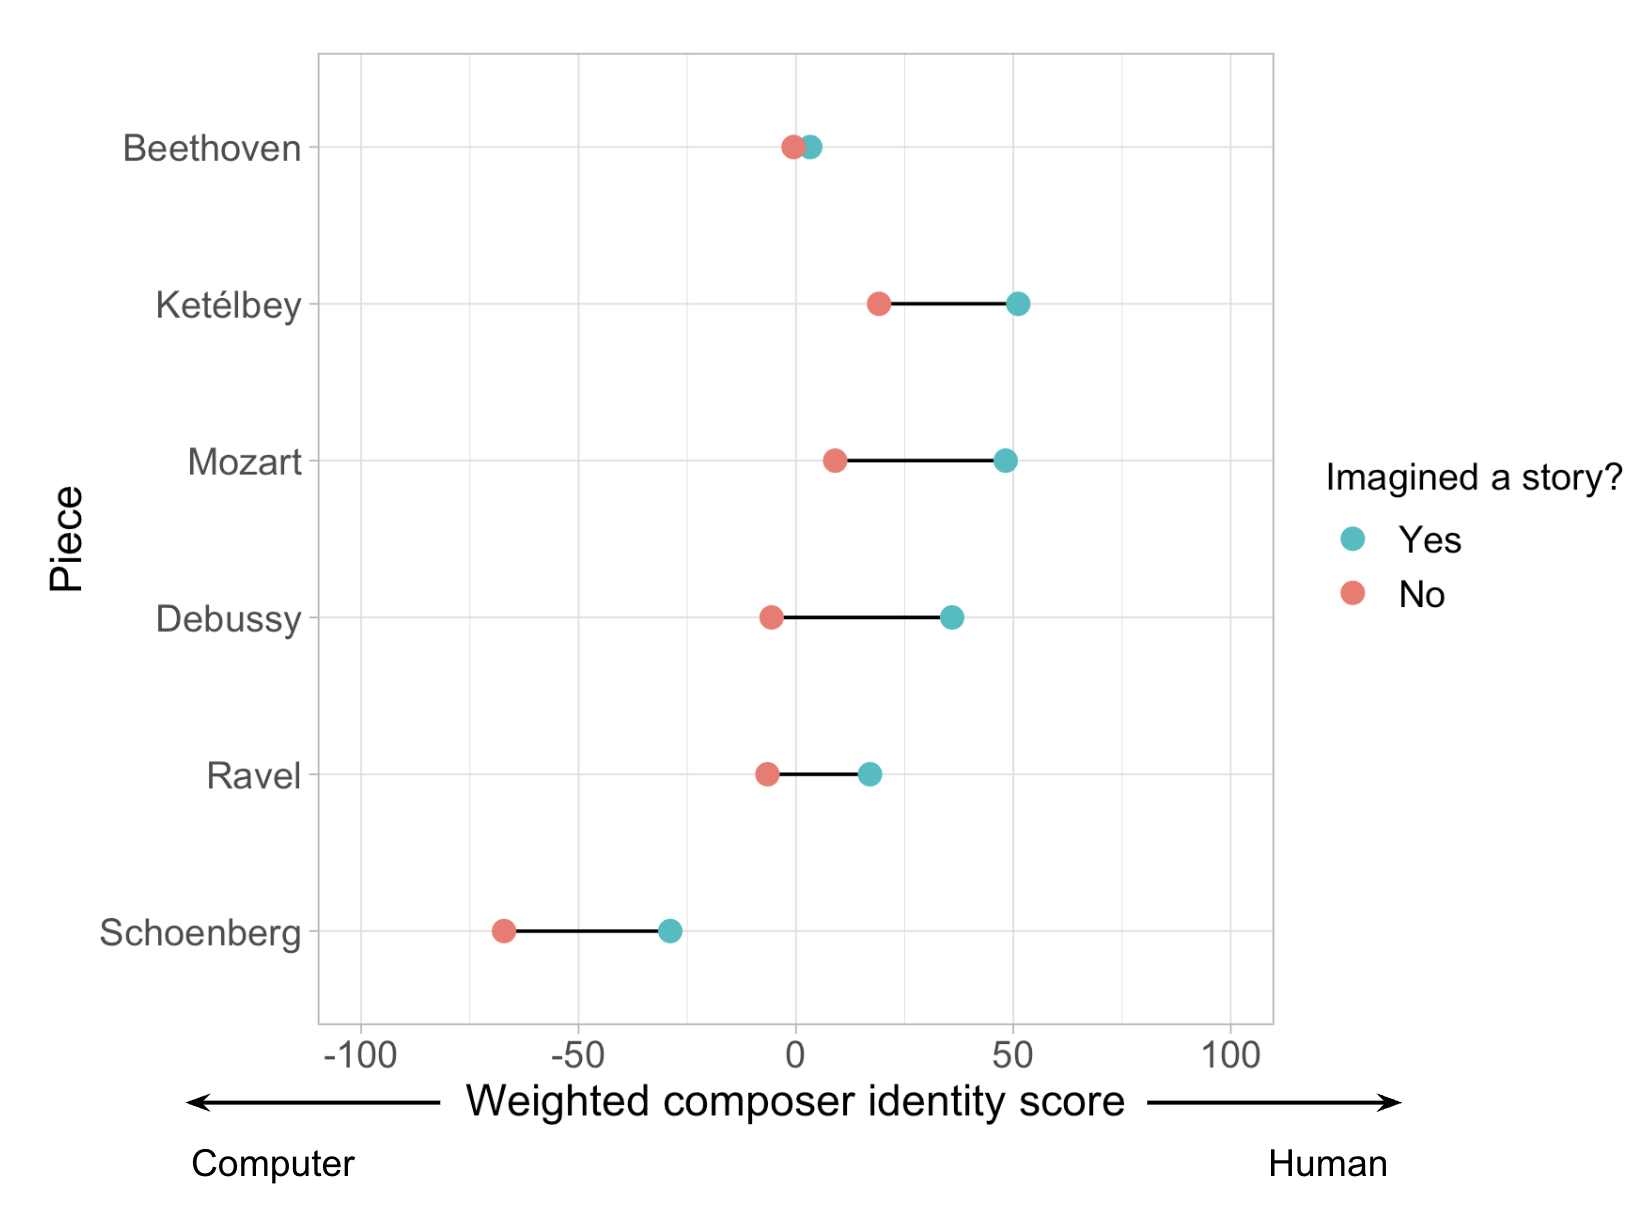
\includegraphics[scale=0.6]{CI_SRQ.png}
	\caption{Mean weighted composer identity scores for each piece, separately for participants who did and did not imagine a story. From top to bottom, pieces are listed in descending order by mean narrativity.}
	\label{fig-ci-differences}
\end{figure}

I also conducted an additional exploratory analysis to examine whether perceived intentionality mediated the relationship between composer identity beliefs and narrativity. In separate regression models across pieces, weighted composer identity scores predicted both SRQ scores ($\beta$ = 0.65, \emph{p} = .003) and intentionality ratings ($\beta$ = 0.52, \emph{p}  \textless .001), and intentionality ratings predicted SRQ scores ($\beta$ = 1.79, \emph{p} \textless .001). These analyses show that perceived intentionality was related to both composer identity judgments and narrativity. When weighted composer identity scores and intentionality were both entered as predictors of SRQ scores (while also controlling for background characteristics and familiarity with the pieces), intentionality was the only significant predictor, ($\beta$ = 1.92, \emph{p} \textless .001); weighted composer identity scores no longer accounted for significant variance in SRQ scores, ($\beta$ = -0.13, \emph{p} = .68). Taken together, these exploratory analyses provide initial evidence that perceived intentionality mediates the relationship between composer identity judgments and narrativity. Figure~\ref*{} shows the standardized regression coefficients for the pairwise relationships between weighted composer identity scores, perceived intentionality, and SRQ ratings.


\subsection{Narrative Engagement}
\subsubsection*{Pre-registered By-Participant Analysis}

For each participant, I regressed the six NE ratings on the corresponding weighted composer identity scores and computed an unstandardized slope coefficient. Positive slopes indicate that NE increased with the perceived humanness of the composer, while negative slopes indicate the opposite relationship. Across participants, the mean slope was positive (\emph{M} = 0.007, \emph{SD} = 0.01), \emph{t}(98) = 4.62, \emph{p} \textless .001, \emph{d} = 0.47. 

\subsubsection*{Exploratory By-Item Analysis}

For each piece, I regressed all participants’ NE ratings on their corresponding weighted composer identity scores. The results of the models are shown in Table 3. For four of the six pieces, greater NE was reliably associated with greater confidence that the piece was composed by a human. For the other two pieces, the relationship was in the same direction but not significant. Across the six pieces, the mean slope was positive (\emph{M} = 0.007, \emph{SD} = 0.004), \emph{t}(5) = 4.34, \emph{p} = .007, \emph{d} = 1.77, corroborating the by-participant analysis. 

\begin{table}[h]
	\centering
	\caption {\emph{By-Item Linear Regression Results in Study 1, Predicting NE from Weighted Composer Identity Scores}} \label{table-CI-NE}
	\bigskip
	\begin{tabular}{c c c c c}
	\toprule
	& Piece and Composer & \emph{b} & \emph{p} &\\
	\hline
	& \emph{Egmont Overture}, Beethoven & 0.002 & .31 &\\
	\hline
	& \emph{In the Mystic Land of Egypt}, Ketélbey & 0.006 & .04* &\\
	\hline
	& \emph{Piano Sonata No. 7}, Mozart & 0.004 & .09 &\\ 
	\hline
	& \emph{En Blanc et Noir}, Debussy & 0.007 & .002** &\\
	\hline
	& \emph{Gaspard de la Nuit}, Ravel & 0.006 & .02* &\\
	\hline
	& \emph{Suite, Op. 29}, Schoenberg & 0.013 & $<.0001$** &\\
	\bottomrule
	\end{tabular}\par
	\bigskip
	\small\textit{}$*p < .05,  \:*\!*p < .01$
	\end{table}

In line with the narrativity analysis, I conducted additional exploratory analyses to examine perceived intentionality as a potential mediator of the observed relationship between composer identity judgments and NE. In separate regression models across pieces, composer identity judgments positively predicted NE, $\beta$ = 0.43, \emph{p} \textless .001, and perceived intentionality, $\beta$ = 0.52, \emph{p} \textless .001, and perceived intentionality predicted NE, $\beta$ = 0.74, \emph{p} \textless .001. These analyses show that perceived intentionality was related to both composer identity judgments and NE. When weighted composer identity scores and intentionality were both entered as predictors of NE (while controlling for background characteristics and familiarity with the pieces), perceived intentionality was the only predictor of NE, $\beta$ = 0.71, \emph{p} \textless .001; composer identity judgments were no longer significant predictors of NE, $\beta$ = 0.03, \emph{p} = .77. As with the narrativity analysis, these exploratory NE analyses suggested that perceived intentionality mediated the relationship between composer identity beliefs and NE.


\subsection{Content of Narratives}

Following my pre-registered analysis plan, I entered participants’ text responses into a plagiarism checker and excluded participants who plagiarized at least one response. While reading through the remaining text responses, I noted responses that were too short or irrelevant to the question (e.g., “I enjoyed the music”) and excluded those as well.

To explore the content of participants’ imagined narratives, I entered each participant’s descriptions of their imagined narratives into the matrix comparison interface of the University of Colorado’s word embedding website (\url{http://wordvec.colorado.edu/matrix_comparison.html}). I selected the word2vec embedding method, which is trained on a large corpus of text from the Google News dataset ($\sim$100 billion words; \url{https://code.google.com/archive/p/word2vec/}). From the site, I obtained cosine similarity scores quantifying the semantic similarity of each pair of stories provided by a given participant. Because the number of imagined stories varied across participants, the number of pairwise comparisons per participant ranged from 1 (for participants who imagined stories for exactly two pieces) to 15 (for participants who imagined stories for all six pieces).

As with the previous aspects of narrative listening, I conducted by-item and by-participant analyses of the narrative content. Because each cosine similarity score from word2vec reflects a pairwise comparison, I analyzed the relationship between these scores and pairwise comparisons of composer identity judgments. To do so, for each of the 15 pairs of pieces in the by-item analysis, I computed the difference between the two pieces in their mean weighted composer identity scores and then assessed the correlation between these difference scores and cosine similarity scores from word2vec. In the by-participant analysis, I computed analogous composer identity difference scores for each participant, separately for each pair of pieces for which they reported imagining a story. As in the by-item analysis, I then assessed the correlation between these difference scores and cosine similarity scores from word2vec. This correlation was positive in the by-item analysis, \emph{r}(13) = .68, \emph{p} = .006, and was also positive (though not significant) in the by-participant analysis, \emph{r}(54) = .13, \emph{p} = .08. Surprisingly, these results indicate that pieces believed to have been composed differently (i.e., by human vs. by computer) seemed to elicit narratives with more similar content. 

The observed relationship in the word2vec analysis may have been a byproduct of the bimodal distribution of weighted CI scores. Despite the 0-to-100 scale of  the confidence question (“How confident are you in your judgment?”) where 0 indicated no confidence (i.e., equal likelihood that the piece was composed by a human or a computer), there were few responses near 0 and many near 50 (see Figure ~\ref*{fig-bimodal-dist}). This distribution suggests that participants may have interpreted 50, rather than 0, as indicating no confidence. 

\begin{figure}[h!tbp]
	\centering
	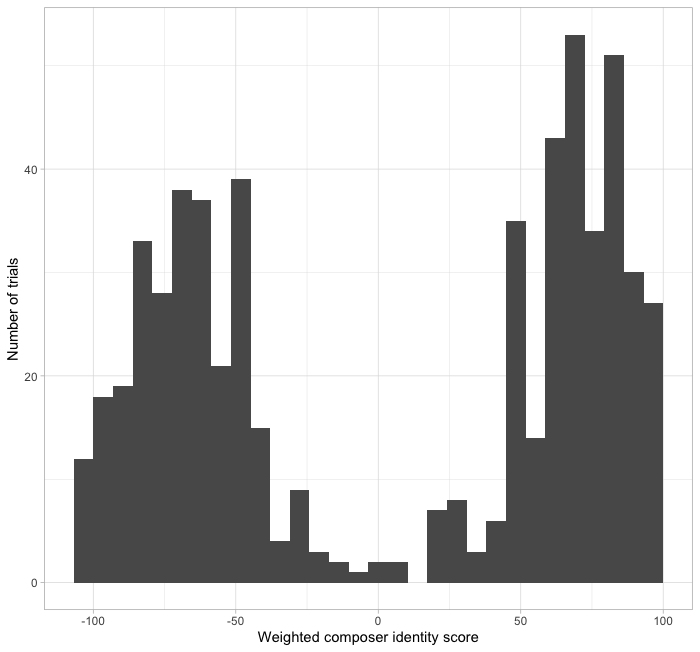
\includegraphics[scale=0.5]{weighted_dist.png}
	\caption{Bimodal distribution of weighted composer identity scores in Study 1.}
	\label{fig-bimodal-dist}
\end{figure}

To further explore the unexpected relationship between CI difference scores and cosine similarity, I examined whether perceived intentionality was related to cosine similarity. This exploratory analysis also allowed me to see if intentionality may have mediated the relationship between CI and narrative content, akin to the main analysis. For each pairwise comparison in the word2vec analysis, I computed the corresponding intentionality difference score. Differences in perceived intentionality were not correlated with cosine similarity scores, \emph{r}(65) = .19, \emph{p} = .13, suggesting that the relationship between CI and cosine similarity was likely spurious.

\section{Discussion}


Study 1 established a correlation between composer identity judgments and numerical narrative listening responses. As the perceived humanness of a composer increased, participants were more likely to imagine a story when listening to music and they reported imagining more vivid narratives. These results are consistent with the possibility that intuitions about composer identity shape the experience of narrative listening.

Importantly, however, stimulus properties of the musical clips could have driven the observed correlations. Features of the music, such as its adherence to a single musical key, may have influenced both participants’ beliefs about the identity of the composer and their narrative listening responses. Therefore, the correlations between composer identity beliefs and narrative listening may have been an artifact of the association between these subjective aspects of music perception and more basic properties of the music.

Moreover, as with any correlational study, many constructs were interrelated. Specifically, beliefs about a composer’s identity seemed to be intertwined with perceptions of intentionality. To determine whether composer identity judgments play a causal role in perceptions of narrative, independent of other factors, in Study 2 I used a true experimental design by experimentally manipulating the information participants received about the composer of each piece of music. This manipulation also addressed the ambiguity of the composer identity judgment questions from Study 1. 

Across participants, each piece of music was presented with a cover story indicating that the piece was composed by either a human or an AI system. If beliefs about a composer’s identity affect narrative listening responses, Study 2 should corroborate the results from the main analysis of Study 1: When pieces are believed to be composed by humans, they should elicit greater narrativity and narrative engagement than when they are believed to be composed by AI. 

\chapter*{Study 2}
\addcontentsline{toc}{chapter}{Study 2}
\chaptermark{Study 2}
\markboth{Study 2}{Study 2}

\section{Method}

I pre-registered my methods and analysis plan on AsPredicted.org (\url{https://aspredicted.org/CK1_1TX})

\subsection*{Participants}

One hundred U.S. participants were recruited from Amazon MTurk via the CloudResearch participant-sourcing platform. All participants had a strong performance record on MTurk ($\ge95\%$ approval on $\ge100$ prior studies). Based on an attention check at the start of the study, three participants were excluded from participating. The mean age of the sample was 41.4 (\emph{SD} = 13.1), with 52\% identifying as male and 47\% as female. Participants reported the following racial/ethnic identities: 81\% White, 10\% African American/Black, 3\% Asian/Asian American/Indian, and 6\% other identities. Across the sample, participants had 0-25 years of experience playing an instrument (\emph{M} = 3.28, \emph{SD} = 5.03) and little experience with music theory (\emph{M} = 1.39 years, \emph{SD} = 2.06). Participants were compensated \$2 for their time. 

\subsection{Materials and Procedure}

The same clips from Study 1 were used. Each music clip was paired with a cover story that described the piece as human- or computer-composed. Pairings were pseudorandomized such that each music clip was framed as human- or AI-composed for half of the participants. In both types of cover stories, the composer was described as having heard/processed many examples of a certain style of music, allowing them/it to identify patterns in the music and emulate a similar style. The cover stories were worded so that the key difference between the human-composed cover story and its computer-composed counterpart was the identity of the composer. The general template of the cover stories was the following:
\\

$[$A human composer wrote/An AI system generated$]$ this piece of music after $[$hearing/being given$]$ many examples of Impressionist piano pieces. $[$He/It$]$ identified patterns among the different pieces to emulate the same exuberant, burbling sound.
\\

For each of the six music clips from Study 1, participants read a cover story and advanced to the next page to hear the corresponding music start playing automatically. On the next page, they were first asked to report the level of intentionality they perceived in the music and then answered all of the narrative listening questions from Study 1. Because participants were explicitly told that each piece was created by either a human or an AI system, the forced-choice question asking for participants’ composer identity judgments and the subsequent question asking for a confidence rating were removed. The familiarity question (“Were you already familiar with this piece?”) was also removed to mitigate demand characteristics. 

As a manipulation check, after answering the narrative listening questions for each piece participants were presented with a forced-choice question asking them to recall the identity of the composer in their assigned cover story (“This is a question to make sure you were paying attention. In the description that preceded this piece of music, it was mentioned that the composer was…”). At the end of the survey, participants were asked to report the extent to which they believed the information about the composers. All other aspects of the procedure were identical to Study 1.

\section{Results}

\subsection{Narrativity}
\subsubsection*{Pre-registered By-Participant Analysis}
For each participant, I computed mean SRQ scores for the pieces they read as being human-composed and AI-composed. Narrativity was numerically greater when participants read that a piece was composed by a human (\emph{M} = 0.56, \emph{SD} = 0.35) than when they read that it was composed by an AI system (\emph{M} = 0.51, \emph{SD} = 0.35), but this difference did not reach significance, \emph{t}(96) = 1.85, \emph{p} = .07, \emph{d} = 0.19.

\subsubsection*{Pre-registered By-Item Analysis}

For each piece, I computed mean SRQ scores for trials in which the piece was framed as human-composed and AI-composed. There was no difference in narrativity between the Human condition (\emph{M} = 0.56, \emph{SD} = 0.12) and the AI condition (\emph{M} = 0.51, \emph{SD} = 0.09), \emph{t}(5) = 1.06, \emph{p} = .34.

\subsection{Narrative Engagement}
\subsubsection*{Pre-registered By-Participant Analysis}
For each participant, I computed mean NE scores for the two conditions. NE was numerically greater when participants read that a piece was composed by a human (\emph{M} = 3.58, \emph{SD} = 1.23) than when they read that it was composed by an AI system (\emph{M} = 3.39, \emph{SD} = 1.30), but this difference did not reach significance, \emph{t}(96) = 1.91, \emph{p} = .06, \emph{d} = 0.08.
\subsubsection*{Pre-registered By-Item Analysis}
In the by-item analysis, there was no significant difference in NE between the Human condition (\emph{M} = 3.57, \emph{SD} = 0.34) and the AI condition (\emph{M} = 3.39, \emph{SD} = 0.33), \emph{t}(5) = 0.93, \emph{p} = .40. 

\subsection{Perceived Intentionality}
Study 1 provided evidence that perceived intentionality mediated the relationship between composer identity beliefs and narrative listening responses. In Study 2, I conducted analogous exploratory analyses to see if the pattern was corroborated (a) with the full sample and (b) excluding trials where participants incorrectly recalled the identity of the supposed composer (12\% of trials). This post-hoc exploratory exclusion was meant to increase the data quality: On trials where participants incorrectly answered the memory check question, they almost certainly did not process the manipulation.

Across participants, the Human condition (\emph{M} = 4.15, \emph{SD} = 1.10) yielded numerically greater intentionality than the AI condition (\emph{M} = 3.92, \emph{SD} = 1.23), \emph{t}(96) = 1.96, \emph{p} = .053. Excluding trials where participants failed to recall the identity of the composer, the difference between the Human (\emph{M} = 4.14, \emph{SD} = 1.11) and AI (\emph{M} = 3.90, \emph{SD} = 1.26) conditions reached significance, \emph{t}(92) = 2.32, \emph{p} = .02, \emph{d} = 0.11\footnote{This exclusion did not change the results for narrative listening.}. When analyzed across pieces with all trials included, intentionality was significantly greater in the Human condition (\emph{M} = 4.15, \emph{SD}  = 0.41) than the AI condition (\emph{M} = 3.92, \emph{SD} = 0.38), \emph{t}(5) = 3.14, \emph{p} = .03, \emph{d} = 0.24. Taken together, these analyses suggest that the experimental manipulation of composer identity affected perceptions of intentionality: The same piece was perceived as expressing greater intention when it was described as having been created by a human, as opposed to an AI system. 

As in Study 1, intentionality was in turn associated with SRQ, $\beta = 1.10, \:p < .001$, and NE, $ \beta = 0.62, \:p < .001$. These results suggest that composer identity beliefs did affect narrative listening, but indirectly through intentionality. Similar to Study 1, I investigated perceived intentionality as a potential mediator of the relationship between composer identity beliefs and narrative listening responses. To do so, I dummy-coded the experimental condition (AI = -1, Human = 1) and entered condition and intentionality into regression models predicting SRQ and NE. With these two predictors in the respective models, only intentionality accounted for unique variance in SRQ scores, $\beta = 1.09, \:p < .001, $and in NE, $ \beta = 0.62, \:p < .001$. 

\subsection{Content of Narratives}
To explore the content of participants’ imagined narratives, I assessed whether word2vec cosine similarity scores differed between composer identity conditions. For each participant, I obtained word2vec cosine similarity scores for each pair of text responses. Comparisons were categorized as “Same-Composer” if both responses were from the Human condition or the AI condition; comparisons were categorized as “Different-Composer” if one response was from the Human condition and one was from the AI condition. Across participants, I computed mean cosine similarity scores for Same-Composer comparisons (\emph{M} = 0.67, \emph{SD} = 0.12) and Different-Composer comparisons (\emph{M} = 0.68, \emph{SD} = 0.11). There was no difference in cosine similarity scores between comparison types, \emph{t}(39) = -0.49, \emph{p} = .62. As in the Study 1 analysis, I also examined the correlation between intentionality difference scores and cosine similarity scores. The two were not correlated, \emph{r}(56) = 0.03, \emph{p} = 0.80.

\section{Discussion}

Although composer identity beliefs predicted narrativity and narrative engagement in Study 1, the experimental manipulation of beliefs in Study 2 did not yield differences on these measures. When participants were told that a given piece of music was composed by a human, they were no more likely to report imagining stories and their imagined stories were no more vivid than when they were told that a piece was composed by an AI system. Furthermore, in the word2vec analysis, participants’ text descriptions of their imagined stories were no more semantically similar to each other for pieces that were framed as having been composed by the same entity (both humans or both AI systems) than for pieces that were framed as having been composed by different entities. 

In the main analysis, however, the Human condition yielded numerically greater narrativity and narrative engagement than the AI condition. This finding is suggestive of the predicted influence of composer identity beliefs. If borne out by future research addressing limitations of the present study (see General Discussion), such an influence would be striking considering that stimulus features of the music were held constant across conditions. Furthermore, perceived intentionality did differ significantly between conditions, and as in Study 1, this measure predicted unique variance in SRQ and NE scores, over and above the manipulation of composer identity beliefs. This finding underscores the power of intentionality beliefs for downstream effects on narrative listening. 

\chapter*{General Discussion}
\addcontentsline{toc}{chapter}{General Discussion}
\chaptermark{General Discussion}
\markboth{General Discussion}{General Discussion}
The present thesis was the first attempt to examine the relationship between beliefs about a musical piece’s composer and the propensity to imagine a story while listening. In Study 1, I investigated this relationship by asking participants to judge who they believed composed a piece of music (Human or AI) and to report their experiences of narrative listening: whether or not they imagined a story (narrativity), the vividness of their story (NE), and the content of their story. In Study 2, I experimentally manipulated composer identity beliefs by presenting participants with a cover story about who composed the music (Human or AI) and asking them to answer the same narrative listening questions. These main variables of interest were seemingly disparate: Composer identity beliefs are a cognitive component of music perception and narrative listening is a complex downstream perceptual effect. 

Nevertheless, in Study 1 composer identity beliefs predicted participants’ likelihood of imagining stories when listening to music, as well as the vividness of their imagined stories, using established measures from previous work (e.g., Margulis et al., 2019). Although these results suggest that composer identity beliefs may shape narrative listening, the experimental manipulation of composer identity beliefs in Study 2 did not significantly affect narrativity or NE. There are a few potential explanations for this null finding. Participants in Study 1 were asked to report their own beliefs as to who composed the music, whereas those in Study 2 were explicitly told what to believe about how each piece of music was created. Thus, on trials in Study 2 for which participants did not believe the cover story, or for which they did not remember the identity of the purported composer, the manipulation may not have been effective. I included a memory check at the end of each trial to try to address this concern, but this was a somewhat crude measure: Of the trials where participants correctly indicated the identity of the composer in the cover story, I could not be certain which reflected genuine processing of the manipulation and which reflected lucky guesses. Excluding trials with incorrect memory check responses improved the data quality, but the difference in narrative listening between the Human and AI conditions remained nonsignificant.

The lack of effect of composer identity beliefs could also be due to the nature of the task. Participants were told about the supposed creation of a piece of music and were then asked seemingly unrelated questions regarding their imagined stories. While this task yielded an association between composer identity beliefs and narrative listening responses in Study 1, the experimental manipulation may have been too far-removed from the narrative listening prompts to yield a causal effect in Study 2. If the manipulation of composer identity had been stronger, perhaps with more details about the human’s or AI’s compositional process, it could have had a downstream effect on narrative listening. However, this could also introduce potential confounds between the two conditions. When writing the Human and AI cover stories, my aim was to keep them as similar as possible to isolate the effect of composer identity beliefs.

Interestingly, perceived intentionality—which participants were asked to report directly after listening to the music—consistently predicted narrative listening responses. In both studies, greater intentionality was associated with higher likelihood of imagining a story and greater narrative engagement across all of the music clips. Furthermore, I observed robust relationships between composer identity beliefs and perceived intentionality, such that when participants spontaneously surmised (Study 1) or were led to believe (Study 2) that a piece was composed by a human, they attributed greater intentionality to it (albeit only significantly in Study 2 when excluding trials with incorrect memory check responses). This suggests that composer identity beliefs can affect narrative listening indirectly through perceived intentionality. Alternatively, the perceived intentionality of an agent—not its identity as a human or AI system per se—may be the key factor governing perceptions of musical narrative (see Abu-Akel et al., 2020). 
 

\section*{Implications}
\addcontentsline{toc}{section}{Implications}
\sectionmark{Implications}
\markboth{Implications}{Implications}

The present research dovetails with studies by Messingschlager and Appel (2022), who investigated narrative transportation—the phenomenon where a reader is completely absorbed into a narrative world—in the context of fictional stories. Like in the present studies, Messingschlager and Appel presented participants with creative works and led participants to believe they were written by either a human or an AI; all of the stories were in fact written by humans. Participants who read that a story was written by an AI reported lower levels of narrative transportation than those who read that the story was written by a human. However, this effect was moderated by the genre of the story: Only for contemporary fiction stories (and not science fiction stories) was narrative transportation lower in the AI condition (Messingschlager \& Appel, 2022). The authors speculated that the lack of a writer identity effect for the science fiction genre may have been due to perceptions of AI as an apt writer for science fiction stories, which are set in technology-rich futures. Participants may have ascribed the supposed AI author with the knowledge or life experience of the world depicted in the science fiction story, thereby eliciting narrative transportation on par with that of a human-written story.

A similar phenomenon may have occurred in the present studies. The majority of participants in Study 1 judged the Schoenberg piece, which is fast and highly dissonant, as having been composed by an AI, and they assigned it correspondingly low SRQ, NE, and intentionality ratings. Interestingly, in Study 2 the ratings for this piece were similarly low in the Human and AI conditions. Like participants in Messingschlager and Appel’s (2022) study who experienced similar levels of narrative transportation when reading a science fiction story regardless of its purported author, participants may have attributed similar levels of narrativity, narrative engagement, and intentionality to the Schoenberg piece across conditions because they conceptualized an AI as an appropriate composer for such a discordant, random-sounding piece. However, without a baseline condition (i.e., no information about the purported creator), I cannot know if the AI condition increased narrative listening for this piece to human-like levels (or if the Human condition reduced narrative listening to AI-like levels for a different reason).

The present research also contributes to the literature on perceptions of narrative across modalities, a type of ‘trans-symbolic comprehension process’ (Steciuch et al., 2023). This cognitive process enables people to form mental models across media (e.g., text, visuals, audio) and stands in contrast to symbol-specific processes (Loughlin et al., 2015), wherein the perceiver mentally represents stimuli in modality-specific ways. Text, for example, is comprehended by decoding words and parsing syntax; music is comprehended by encoding pitches and volume. In Steciuch et al.’s (2023) exploration of trans-symbolic comprehension, participants were asked to type out their thoughts while reading stories and viewing paintings. Their responses were coded for various trans-symbolic comprehension processes, including observations about explicit content, inferences that connected multiple components of the stimulus, and statements that extended past information presented in the text or painting. Positive correlations were observed between the prominence of these processes across text and paintings, suggesting that certain comprehension mechanisms aid high-level, cross-modal construals.

Trans-symbolic comprehension also has a neural basis. In an fMRI study by Nguyen et al. (2019), one group of participants watched a video depicting a complex narrative involving geometric shapes and another group listened to a reading of the concrete events from the same narrative. Participants were asked to verbally recall the events of their assigned narrative in as much detail as possible. The more similar any two participants’ spontaneous interpretations of the narrative (measured through latent semantic analysis), the more similar their responses were in two areas of the brain: the default mode network (DMN)—which supports mental state attribution and narrative processing—and the fronto-parietal network—which supports cognitive control and attentional processes.

The perception of narrative seems to transcend any particular symbol system. At a broad level, mentally modeling a narrative involves understanding a ‘system of signs’ that changes over time (Almén, 2008). Music, like language, is made up of individual units (notes or phonemes) that can be perceived in terms of broader groupings (e.g., phrases). When perceiving musical narratives specifically, listeners may consider the extent to which the music imitates extramusical sounds, metaphoric associations between structural components of the music and emotional experiences, cultural conventions, and personally-relevant associations (Trainor \& Trehub, 1992). 

In line with previous research (e.g., Hong et al., 2022; Steinbeis \& Koelsch, 2009), the present thesis demonstrates that beliefs about human and AI composers are associated with music perception. Specifically, when participants judged a piece as more likely to have been composed by a human, they were more likely to imagine a story in response to the music and their stories were more engaging. This finding is consistent with Hong et al. (2022), who found that when AI music generators were depicted in an embodied robotic form and described as having humanlike traits, they were more likely to be accepted as musicians, which in turn led to more positive evaluations of AI-composed music. Critically, in Studies 1 and 2 the intentionality with which a piece was perceived to have been composed seemed to mediate this relationship. This aligns with research showing that merely believing that a piece of music was composed by a human (versus a computer) elicits greater activity in neural areas implicated in mental state attribution (Steinbeis \& Koelsch, 2009). In light of the present results, several outstanding questions remain that can be addressed in future research. 



\section*{Limitations and Future Directions}
\addcontentsline{toc}{section}{Limitations and Future Directions}
\sectionmark{Limitations and Future Directions}
\markboth{Limitations and Future Directions}{Limitations and Future Directions}

The present thesis bridged research on empirical aesthetics, human-computer interaction, and music perception. Because of its novelty, it was difficult to anticipate the effectiveness of the cover stories across the music clips. Descriptive statistics from the item analysis suggest that the cover stories functioned differently across the six pieces. For example, in Study 2 narrativity was higher in the Human condition than the AI condition for the music by Mozart, Beethoven, and Ravel. In contrast, narrativity was almost the same across the two conditions for the piece by Schoenberg, and was slightly greater in the AI condition than the Human condition for the music by Ketélbey and Debussy. Margulis et al. (2019) consulted with music theorists to quantify the stimulus features of the music clips in their study, specifically in terms of contrast and topicality. Because I rendered their clips in a synthesized format, I could not use those metrics to explain why the cover stories yielded such varied judgments of composer identity and narrative listening responses across pieces. Aside from contrast and topicality, the pieces also vary on a set of more basic dimensions (e.g., tempo, harmonic progression, dynamic contrast). Without a model of these dimensions of the music, and how the pieces relate to each other along these dimensions, it is difficult to know what participants picked up on when they judged certain pieces of music as more human-sounding or more AI-sounding. Future research in this domain might collect information about the perceptual features of music to understand their contributions relative to those of higher-level factors like beliefs about composer identity. 

The present thesis was also limited in its text analysis. In line with previous work, (Margulis et al., 2022b), I prompted participants to describe their imagined narratives in as much detail as possible. However, because this was such an open-ended prompt, the text responses varied greatly in terms of length and syntax. The sheer number of unique words reported, in combination with the relatively small sample size imposed by restrictions of the word2vec analysis (e.g., only responses from participants who imagined at least two stories could be analyzed), made it difficult to discern clear patterns. While this open-ended question may have been effective for Margulis et al.’s (2022b) examination of broad, cultural differences in perceptions of musical narrative, it may be too general for the more subtle manipulation of composer identity beliefs. Moreover, word2vec may not be the best tool to analyze participants’ imagined stories. Although the model quantifies the similarity of texts relative to each other, its absolute cosine similarity scores are difficult to interpret and do not provide insight into the semantic content of the text. Studies that build upon this research using a similar word embedding model might include a more focused prompt to probe the content of narratives. Dictionary-based approaches, such as Linguistic Inquiry and Word Count (LIWC; Tausczik \& Pennebaker, 2010), may be a useful supplement for quantifying the prevalence of certain kinds of words for each imagined story.

A downside to asking participants to self-report their imagined stories after the music clip has played is that this requires memory of how the music sounded. Furthermore, these reports do not contain information about when participants heard each of the events of their imagined stories—an important aspect of narrative. To investigate this, future studies could prompt participants to indicate each time they hear a new event in the music’s narrative, in real time (Margulis et al., 2022a). If event perception tracks with the aspects of narrative listening investigated in the present thesis (narrativity and narrative engagement), then participants who share beliefs about the composer’s identity should show greater consensus in the timing of the events than participants with different beliefs. 

The manipulation of composer identity beliefs provides another opportunity for extension of the present research. Study 2 included only two composer identity conditions, which does not account for degrees of autonomy of the AI system. Depending on the AI system, humans have varying levels of involvement: AI systems that rely on supervised learning, for example, require human feedback to improve their performance. It would also be interesting to understand how people perceive collaborations between human and AI composers. For example, a human might input an initial musical idea, the AI might generate a music clip based on that input, and the human might refine the AI’s creation to achieve something greater than what each entity can create on its own. Such collaboration has the potential to stimulate human creativity by expanding the range of compositional possibilities (see Carter et al., 2017; Esling \& Devis, 2020). 

In the same vein, future research should consider humans’ intuitions about what certain kinds of music usually sound like and the quality of an AI system’s execution of the music. Rather than reporting imagined stories, participants could provide text descriptions of narratives as an input to an AI system. The system’s musical outputs could be rated by another group of participants for the effectiveness with which they convey the musical narrative. ChatGPT, a large language model, already has the ability to recommend musical properties that would be appropriate for the user’s specified music. As shown in Figure ~\ref{fig-chatgpt}, when a narrative is inputted, ChatGPT suggests a number of musical properties that could feasibly suit it.

\begin{figure}[h!tbp]
	\centering
	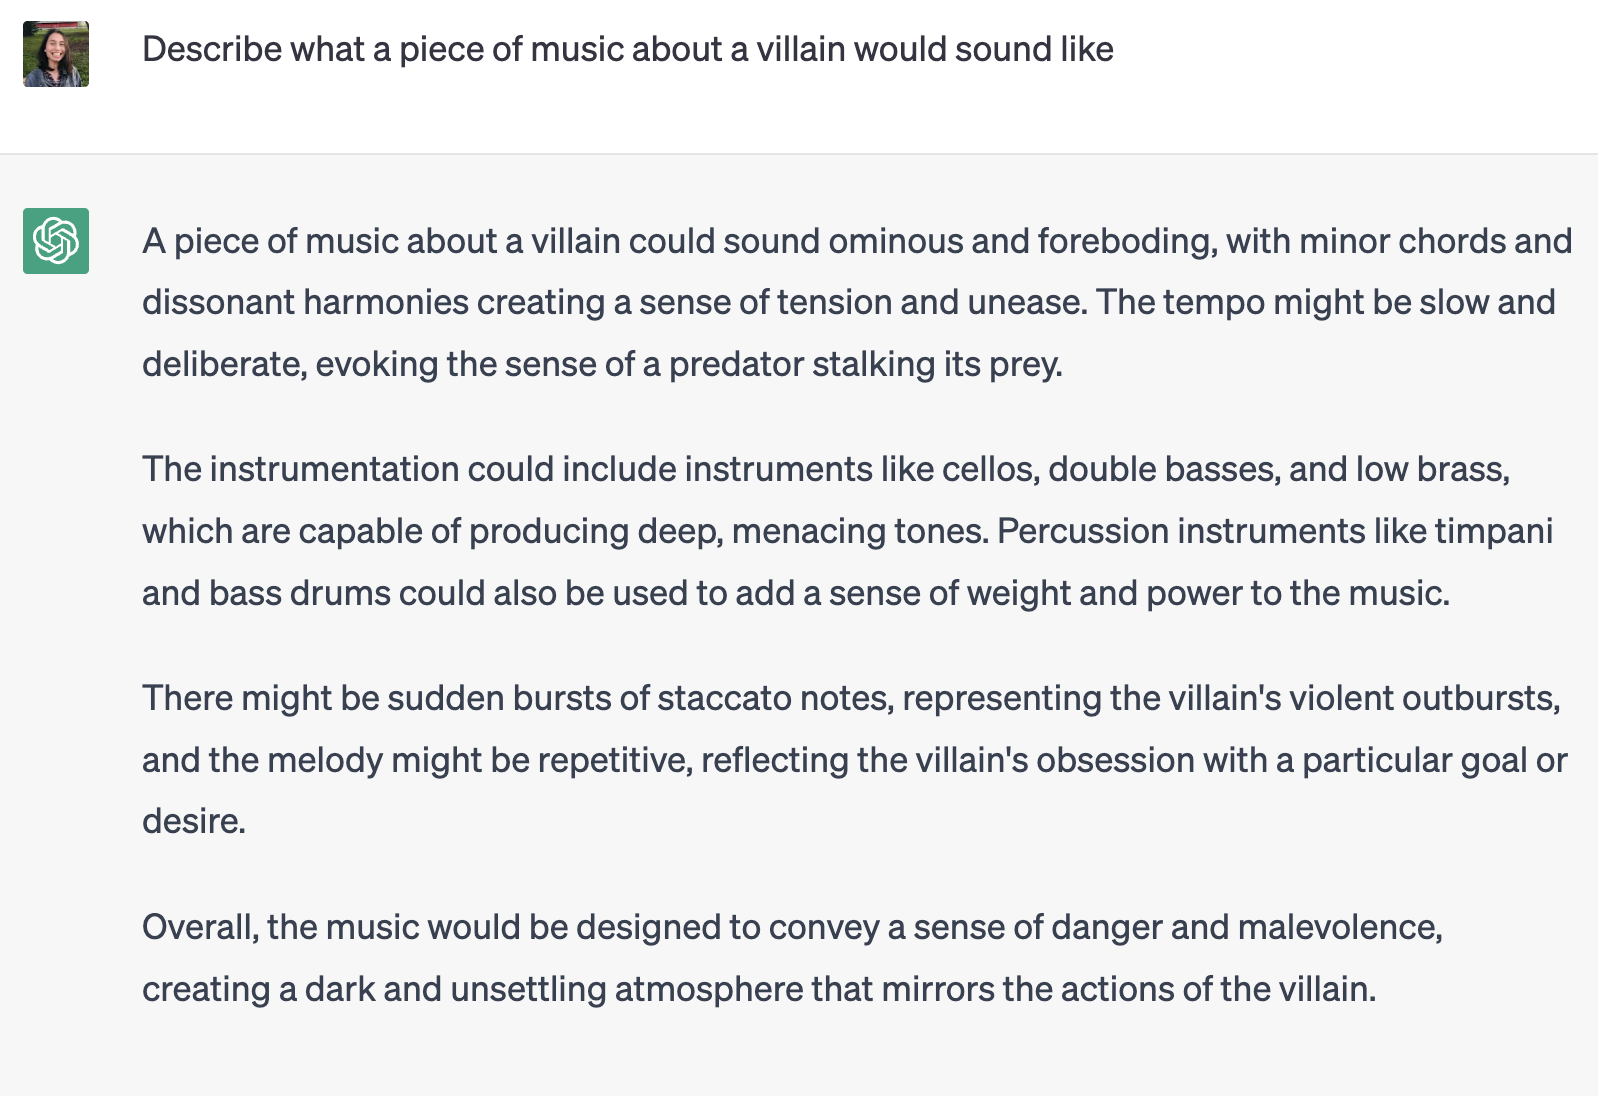
\includegraphics[scale=0.6]{chatgpt.png}
	\caption{ChatGPT's recommendations for musical properties that would evoke images of someone being chased.}
	\label{fig-chatgpt}
\end{figure}

Musical properties recommended by ChatGPT could be compared to those generated by participants, which could reveal the degree of consensus between AI and humans' conceptions of a particular musical narrative. 

Another possible avenue for future research would be to manipulate levels of perceived intentionality attributed to the composer, similar to research on visual art (Jucker et al., 2014). For example, in a ‘low-intention’ condition a piece of music could be described as the product of a composer testing out new compositional ideas. In contrast, a ‘high-intention’ description of the same piece of music might describe events in the composer’s life that led to certain compositional choices for the piece. Such an experimental manipulation would target the construct of intentionality, rather than the agent associated with it, and address the underlying assumption that humans are perceived as more intentional than AI systems. Rather than mediating effects of composer identity beliefs on narrative listening, perceived intentionality may have a causal impact on both of these other aspects of music perception.

\section*{Conclusion}
\addcontentsline{toc}{section}{Conclusion}
\sectionmark{Conclusion}
\markboth{Conclusion}{Conclusion}

As AI music generators continue to advance, questions of the artistic merit of their compositions will persist (Boden, 2010; Dahlstedt, 2021). The conversation around AI’s creative capabilities tends to be bleak, focusing on the declining value of human artists. But as with many other technologies that were met with initial resistance, such as the camera (Teicher, 2016) and musical synthesizers (Esling \& Devis, 2020), AI systems can be seen as an opportunity to augment humans’ creative capabilities. Rather than limit AI systems according to human preconceptions of creativity, it may be more productive to take advantage of their rapid and seemingly boundless generativity. 

Regardless of the tools used to create a work of art, the intentionality of the artist will surely play an important role in shaping aesthetic responses. The field of cognitive science—which draws upon many disciplines including philosophy, artificial intelligence, and psychology to understand the nature of mental life—is well-equipped to articulate the definition of intentionality and how it manifests in both human and computer minds. To understand experiences that we hold dear as unique to humans, like storytelling and music, we must continue to study broad notions like intentionality that guide our remarkable human propensity to make meaning. 


% %If you feel it necessary to include an appendix, it goes here.
%     \appendix
%       \chapter{The First Appendix}
%       \chapter{The Second Appendix, for Fun}


%This is where endnotes are supposed to go, if you have them.
%I have no idea how endnotes work with LaTeX.

  \backmatter % backmatter makes the index and bibliography appear properly in the t.o.c...

% if you're using bibtex, the next line forces every entry in the bibtex file to be included
% in your bibliography, regardless of whether or not you've cited it in the thesis.
    \nocite{*}

% Rename my bibliography to be called "Works Cited" and not "References" or ``Bibliography''
% \renewcommand{\bibname}{Works Cited}

%    \bibliographystyle{bsts/mla-good} % there are a variety of styles available; 
%  \bibliographystyle{plainnat}
% replace ``plainnat'' with the style of choice. You can refer to files in the bsts or APA 
% subfolder, e.g. 
 \bibliographystyle{APA/apa-good}  % or
 \bibliography{thesis}
 % Comment the above two lines and uncomment the next line to use biblatex-chicago.
 %\printbibliography[heading=bibintoc]

% Finally, an index would go here... but it is also optional.
\end{document}
